\chapter{Conception et implémentation}
\label{chapterImpl}

Ce chapitre traitera de ce qui a été conçu, et implémenté durant le stage.
\section{Technologies utilisées}
Les technologies étaient fixées d'avance par les contraintes du projet.

\begin{itemize}
	\item Le langage de programmation est le \brand{C++}.
	\item Les cadriciels utilisés sont \brand{Qt} pour l'interface et \brand{Jamoma} pour la bibliothèque de base.
	\item La majorité du développement se fait sous \brand{Mac OS X}.
	\item Les outils de gestion de projet sont \brand{Dropbox}, \brand{GitHub} et \brand{Asana}.
\end{itemize}

Néanmoins, très tôt j'ai décidé d'entreprendre un portage des librairies nécessaires sous systèmes \brand{Linux}, de manière à pouvoir faire fonctionner le logiciel sur systèmes embarqués.

\section{Organisation du travail}
\subsection{Choix effectués}
PetriNet API
ZeroConf
\section{Réalisations}
\subsection{Logiciel de test de répartition}
Ma première impulsion a été de créer un logiciel, nommé \brand{dpetri} (pour \textit{distributed petri}) qui permette d'exécuter un réseau de Petri sur un réseau informatique, en associant à chaque machine du réseau des transitions (la valeur des places est partagée intelligemment entre les deux nœuds qui y sont attenants).

Les échanges de messages se font par \ac{OSC}, et il n'y a pas de gestion du retard intégrée. Cette tâche reste à appliquer à la main, ou avec un algorithme externe, sur les réseaux de Petri passés en entrée.

La librairie sous-jacente utilisée était à la base \brand{PetriNet API}~\cite{lohmann2009petri}. Néanmoins, en voulant tester sur \brand{Android}, la librairie n'a pas pu fonctionner car elle requiert un fichier binaire propriétaire, qui n'est compilé que pour architectures \brand{x86}. J'ai donc réimplémenté une structure de réseau de Petri qui suit l'architecture de \brand{PetriNet API}, mais en offrant uniquement les capacités nécessaires au logiciel. Ceci dit, la visualisation en temps-réel n'est alors plus possible.

Le logiciel affiche le retard à l'exécution d'une transition. L'interface, visible en \cref{fig.dpetri}, est écrite en \brand{Qt}, et utilise \brand{ZeroConf} avec une architecture client / serveur.
\begin{figure}[H]
	\centering
	\begin{tabu} to \linewidth {cc}
	\begin{subfigure}{.5\textwidth}
		\centering
		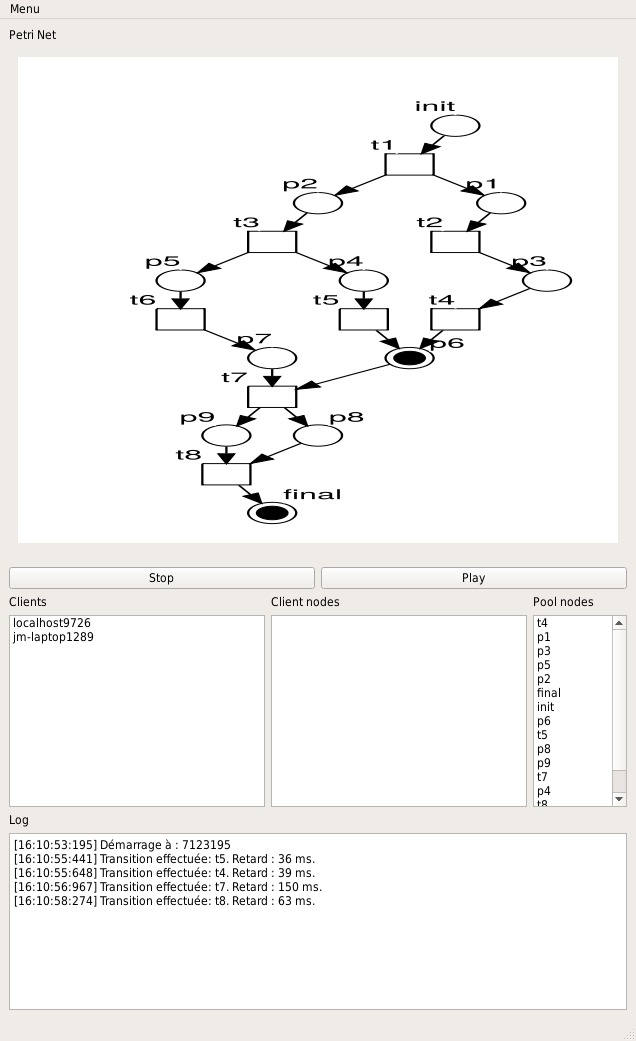
\includegraphics[scale=0.3]{images/dpetriServer.png}
		\caption{Vue serveur}
	\end{subfigure} &
	\begin{subfigure}{.5\textwidth}
		\centering
		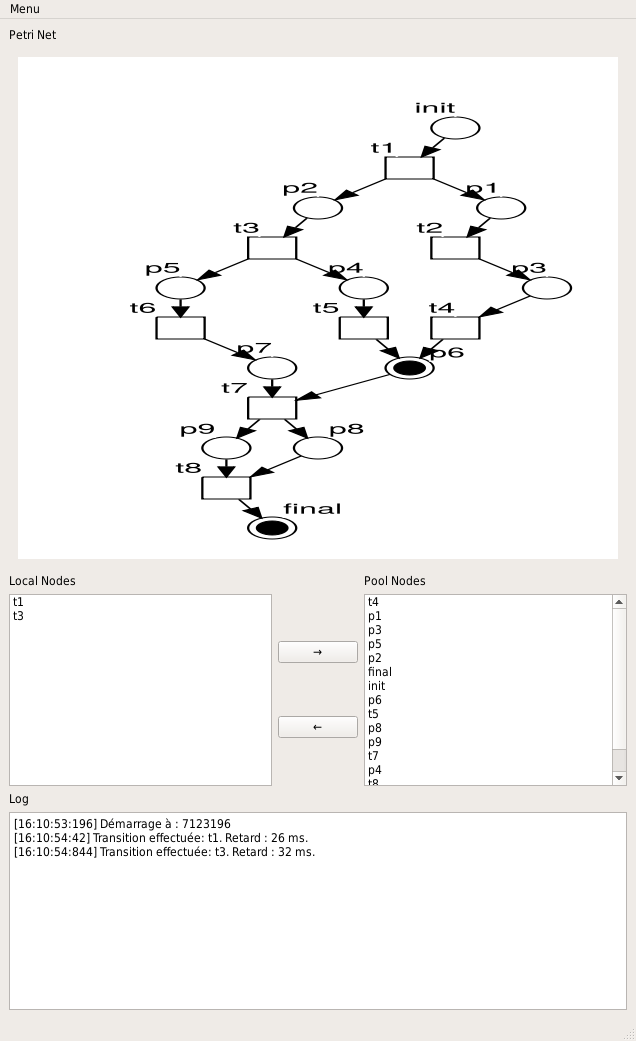
\includegraphics[scale=0.3]{images/dpetriClient.png}
		\caption{Vue client}
	\end{subfigure}
	\end{tabu}
	
	\begin{subfigure}{.5\textwidth}
		\centering
		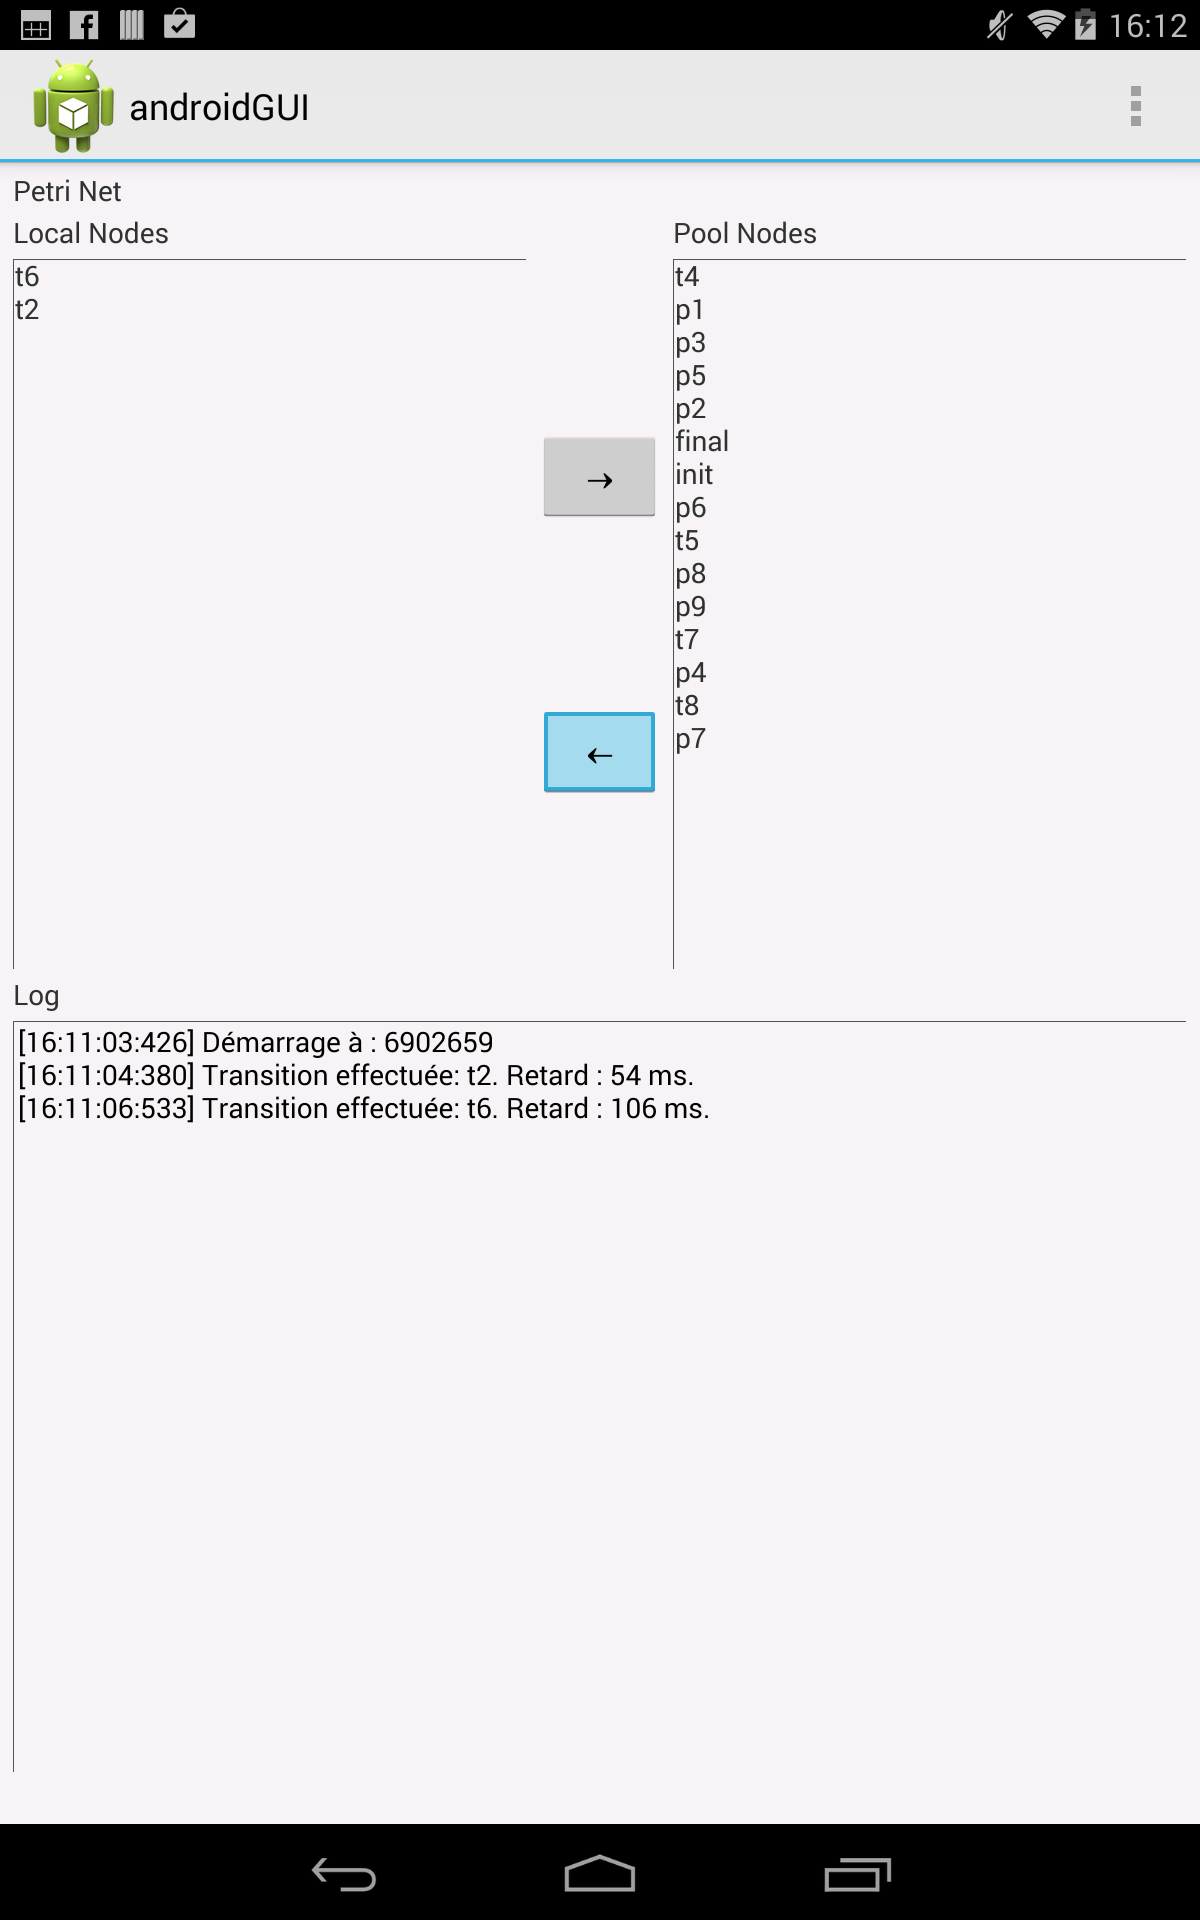
\includegraphics[scale=0.16]{images/dpetriAndroid.png}
		\caption{Vue client Android}
	\end{subfigure}
	
	\caption{Présentation des différentes vues du logiciel de test, \brand{dpetri}}
	\label{fig.dpetri}
\end{figure}

Le code source est présent sur \brand{GitHub} à l'adresse \url{https://github.com/jcelerier/dpetri}.

\subsection{Portage sous GNU/Linux et Android}
Afin d'avoir une exécution des scénarios interactifs sur embarqué, il était nécessaire de porter \brand{Jamoma} et \brand{i-score} sous systèmes Linux (\brand{Android} étant très semblable).

Cela a nécessité un portage du processus de construction logicielle (\textit{build system})  de \brand{Jamoma}, un script Ruby personnalisé, vers \gls{CMake}.

Réaliser ce développement a aussi permis de distribuer \brand{i-score} sous \gls{macports}, et a ouvert de nouvelles perspectives de développement pour l'embarqué sur le logiciel; de plus, un système d'\gls{contintegr} est désormais envisageable.

Un portage a aussi été réalisé sous \brand{BeagleBoard}, pour offrir un \textit{proof-of-concept} de fonctionnement sur périphérique embarqué courant. Cependant, le moteur d'exécution d'\brand{i-score}, travaillant à une fréquence de $\num{1} \si{\kHz}$.

J'ai travaillé sur les branches \texttt{feature/cmake} des projets \texttt{Jamoma/JamomaCore}, \texttt{OSSIA/Score} et \texttt{i-score/i-score} sur \brand{GitHub}.
\subsection{Implémentation dans l'API OSSIA}
L'\brand{API} expose les éléments du paradigme \brand{OSSIA} : 
\texttt{
\begin{itemize}
	\item Boîtes
	\item Processus
	\item Scénarios
	\item Évènements
	\item Branchements conditionnels
\end{itemize}
}

Les notions qui ont été ajoutées sont celles de \texttt{Groupes, Permissions, Clients, Sessions}.

Le code source se situe sur \brand{GitHub}, à l'adresse \url{https://github.com/jcelerier/ScoreNetApi}.

L'idée principale est qu'un client peut avoir différentes permissions sur un groupe, explicitées en \cref{tbl.permissions}.

\begin{table}[H]
	\centering
	
	\begin{tabu} to \linewidth{XX[4,m]}
		\textbf{Visualisation} & Le client reçoit les changements sur les scénarios compris dans ce groupe. \\ \midrule
		\textbf{Écriture} & Le client envoie les changements qu'il réalise sur les scénarios compris dans ce groupe. \\ \midrule 
		\textbf{Exécution} & Le client exécute le contenu des scénarios compris dans ce groupe. \\
	\end{tabu}
	
	\caption{Explication des permissions possibles}
	\label{tbl.permissions}
\end{table}

Les permissions d'écriture et d'exécution impliquent la permission de visualisation.

\subsubsection{Session}
Une session est ce qui identifie un groupe de machines travaillant sur le même document.

Il existe deux types de sessions : les sessions maîtresses et les sessions clientes.
Des sessions clientes se connectent à une session maîtresse, généralement la première machine à être lancée, ou la plus puissante.

Une session maîtresse sert principalement à : 
\begin{itemize}
	\item Avoir une vue maîtresse, permettant d'écrire sur tous les groupes.
	\item Avoir une adresse à laquelle se connecter.
	\item Mettre en relation les clients entre eux.
	\item Vérifier si les clients sont toujours connectés.
	\item Éventuellement avoir un rôle de validation des données échangées, amis cela n'a pas été implémenté.
\end{itemize}

\subsubsection{Groupe}
Des scénarios sont assignés à un groupe.

Comme il a pu être vu en \cref{fig.RepartOSSIA}, la méthode visuelle recommandée pour différencier des groupes est la couleur.

Un groupe peut aussi être mis en sourdine, que ce soit au niveau local (sur une seule machine), ou au niveau de la session (sur toutes les machines). Cela signifie que ses processus ne s'exécutent plus.

Enfin, l'idée d'un groupe spécial dédié à la sauvegarde (\textit{backup}) est proposée : dans ce groupe, les clients sont par défaut mis en sourdine, à l'exception d'un seul. Si lors de l'exécution un des clients ne répond plus, la session maîtresse enlève sa sourdine à un autre client.

Un groupe possède de plus certaines fonctionnalités d'agrégation des clients qui l'exécutent, via l'exposition d'une interface en \ac{OSC}.

L'interface proposée est la suivante : (\texttt{group} peut être remplacé par le nom du groupe, mais cela pose problème car il faut alors interdire les caractères spéciaux et les espaces).

En écriture sur le groupe : 
\begin{itemize}
	\item /group/enable/fonctionnalité
	\item /group/disable/fonctionnalité
	\item /group/parameter/nomDuParamètre id
\end{itemize}

Émis par le groupe :
\begin{itemize}
	\item /group/connexions
	\item /group/nomDuParamère/fonctionnalité
\end{itemize}
\subsection{Implémentation dans le logiciel i-score}
\subsection{Démonstration dans le cadre d'un vrai scénario}
